\section{FairTest}
\label{sect:fairtest}

% What we built

To address the descrimination test, We designed \textit{FairTest}, a software
testing framework for web-based applications to find out potential
\textit{privacy bugs}, whose definition was just described. The framework
records both the input and output of an application, and based on the
correlation between the output and certain protected private data (such as
gender, race, etc.), discover if any \textit{privacy bugs} can be discovered 
based on the statistical parity model.

% Target user / characteristic

\textit{FairTest} is designed to be used for designers and engineers of 
data-based web applications. In addition, it can also be used for auditors 
or government agencies to look for evidence on certain parity violation,
such as in the Staples case. The framework, for generality, is interfaced 
with RESTful API that can easily connect to existing software solutions.
We expect that developers will only make minimal modifications to the
application (mostly adding the tracking code) to derive the data for audit
in \textit{FairTest}. The framework itself is implemented in Python and
Django, with support to both SQLite or PostgreSQL database.

% Data got

Once \textit{FairTest} has information about the users and the corresponding
outputs from the software being tested, it can generate statistical reports
evaluating the statistical parity between the protected info, the actual
input and the output. This info can then be reported either through a RESTful
API or a web interface to the developer or tester. With the info, we can then
suggest potential \textit{privacy bugs} that are caused by the statiscal
parity found by the system, offering suggestion to the developer if the
customization engine appears acceptable or not.

% Subsections

This section will be divided into the following parts. In subsection 3.1, the
\textit{FairTest} archetecture will be discussed; and subsection 3.2 will
discuss the API design of \textit{FairTest}. 

\subsection{Architecture}

% Overview
The \textit{FairTest} architecture contains three most important parts: the
input API, the data analyzer and the result reporter. Together with an
application, the architecture is shown in Figure~\ref{fig:FairtestArch}.

\begin{figure}[h]
 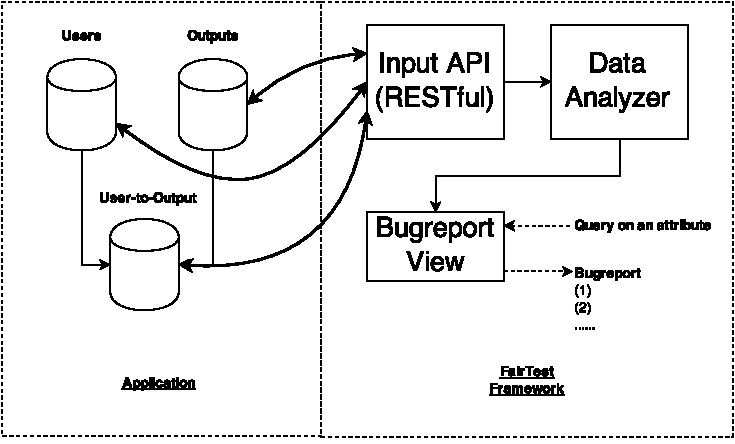
\includegraphics[width=0.49\textwidth]
  {\detokenize{figures/architecture}}
  \caption{\textbf{FairTest Architecture}. The diagram shows a very simple
  application hooked up with the FairTest architecture. Bold lines are API
  calls to be added by the developer to the application code, and dash lines
  are used by the auditors to get the result. Solid line shows data flow
  as part of the application or testing framework.}
  \label{fig:FairtestArch}
\end{figure}

In the figure, it shows that the input API is derectly linked with the 


\subsection{API}
Describe maybe with a table
\begin{itemize}
  \item Describe
  \item Explain why we think it is a good API? (e.g., is it extensible?)
\end{itemize}
